\begin{figure}[ht]
	\centerline{
	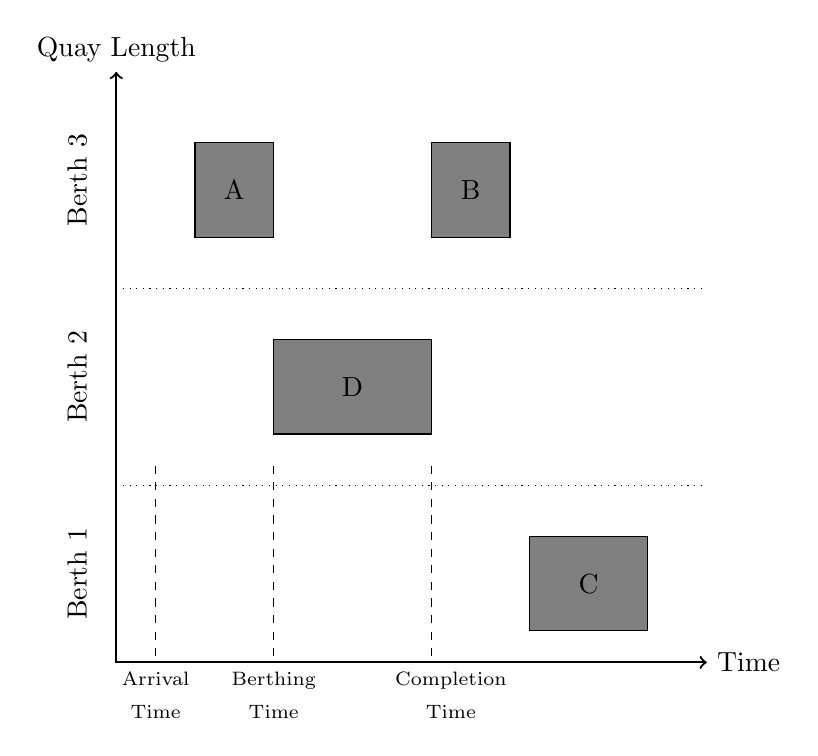
\begin{tikzpicture}[scale=0.5]
        \draw [thick,<->] (0,15) node[above]{Quay Length} --
                                 (0,0)                    --
                                 (15,0) node[right]{Time};
        \node[rectangle, draw, fill=gray, minimum width=1cm, minimum height = 1.2cm] at (3,12) {A};
        \node[rectangle, draw, fill=gray, minimum width=1cm, minimum height = 1.2cm] at (9,12) {B};
        \node[rectangle, draw, fill=gray, minimum width=2cm, minimum height = 1.2cm] at (6,7) {D};
        \node[rectangle, draw, fill=gray, minimum width=1.5cm, minimum height = 1.2cm] at (12,2) {C};

	\node [below,align=center] at (1.0,0) {\scriptsize Arrival\\ \scriptsize Time};
	\draw[dashed] (1.0,5)--(1.0,0);

	\node [below, align=center] at (4,0) {\scriptsize Berthing\\ \scriptsize Time};
	\draw[dashed] (4,5)--(4,0);

	\node [below, align=center] at (8.5,0) {\scriptsize Completion\\ \scriptsize Time};
	\draw[dashed] (8,5)--(8,0);

        \draw[dotted] (0, 4.5) -- (15, 4.5);
        \draw[dotted] (0, 9.5) -- (15, 9.5);

	\node[rotate=90] at (-1, 2.25) {Berth 1};
	\node[rotate=90] at (-1, 7.25) {Berth 2};
	\node[rotate=90] at (-1, 12.25) {Berth 3};

	\end{tikzpicture}
    }
	\caption{The representation of the berth-time space}
	\label{fig:bap}
\end{figure}